\documentclass[aspectratio=139,8pt]{beamer}
\usepackage[utf8]{inputenc}
\usepackage[T1]{fontenc}
\usepackage[french]{babel}
\usepackage{amsmath,amssymb}
\usepackage{algorithm}
\usepackage{algorithmic}
\usepackage{tikz}
\usetikzlibrary{positioning,shapes,arrows}
\usetheme{Madrid}
\usecolortheme{whale}
\usefonttheme{professionalfonts}
\setbeamertemplate{navigation symbols}{}
\setbeamertemplate{headline}{}
\setbeamertemplate{footline}[frame number]
\hfuzz=50pt

\newcommand{\minPts}{\mathrm{minPts}}
\tikzstyle{block} = [rectangle, draw, rounded corners, align=center, minimum height=8mm, minimum width=18mm]

\title[HDBSCAN]{Présentation de l'algorithme HDBSCAN}
\subtitle{Hierarchical Density-Based Spatial Clustering of Applications with Noise}
\author[T. Randriamamonjy \& E. Zamanileha]{Randriamamonjy Tokiniaina \and Zamanileha Elorgin Fernando}
\date{13 octobre 2025}
\institute[Université d'Antananarivo]{Université d'Antananarivo, Facultés des sciences, Département des Mathématiques}

\begin{document}

% Page de titre
\begin{frame}
\titlepage
\end{frame}

% Table des matières
\begin{frame}{Plan de la présentation}
\tableofcontents
\end{frame}

\section{Introduction}

\begin{frame}{Qu'est-ce que HDBSCAN ?}
\begin{block}{Définition}
HDBSCAN est un algorithme de \textbf{regroupement hiérarchique basé sur la densité} qui étend DBSCAN :
\begin{itemize}
\item Transforme DBSCAN en algorithme hiérarchique
\item Extraction automatique de clusters plats basée sur la \textbf{stabilité}
\item Gère des clusters de densités variables
\item Robuste au bruit et aux valeurs aberrantes
\item Pas de paramètre $\varepsilon$ fixe (contrairement à DBSCAN)
\end{itemize}
\end{block}

\begin{alertblock}{Avantages clés}
\textbf{Campello, Moulavi \& Sander (2013)} : Détection automatique du nombre de clusters, pas de seuil de densité unique.
\end{alertblock}
\end{frame}

\section{Étapes de l'algorithme}

\subsection{1. Représentation des données initiales}

\begin{frame}{1. Représentation des données}
\begin{itemize}
\item Données : Ensemble $D$ dans un espace métrique $(D, d)$
\item Distance : $d(x, y)$ entre points
\item Objectif : Identifier des régions de haute densité
\end{itemize}

\begin{figure}
\centering
% \begin{tikzpicture}[scale=0.6]
% \fill[blue!30] (0,0) circle (0.5);
% \fill[blue!30] (1,0) circle (0.5);
% \fill[blue!30] (0.5,1) circle (0.5);
% \fill[red!30] (4,0) circle (0.5);
% \fill[red!30] (5,1) circle (0.5);
% \fill[red!30] (4.5,0.5) circle (0.5);
% \fill[gray!30] (2,2) circle (0.3);
% \node at (2,-1) {Données initiales};
% \end{tikzpicture}
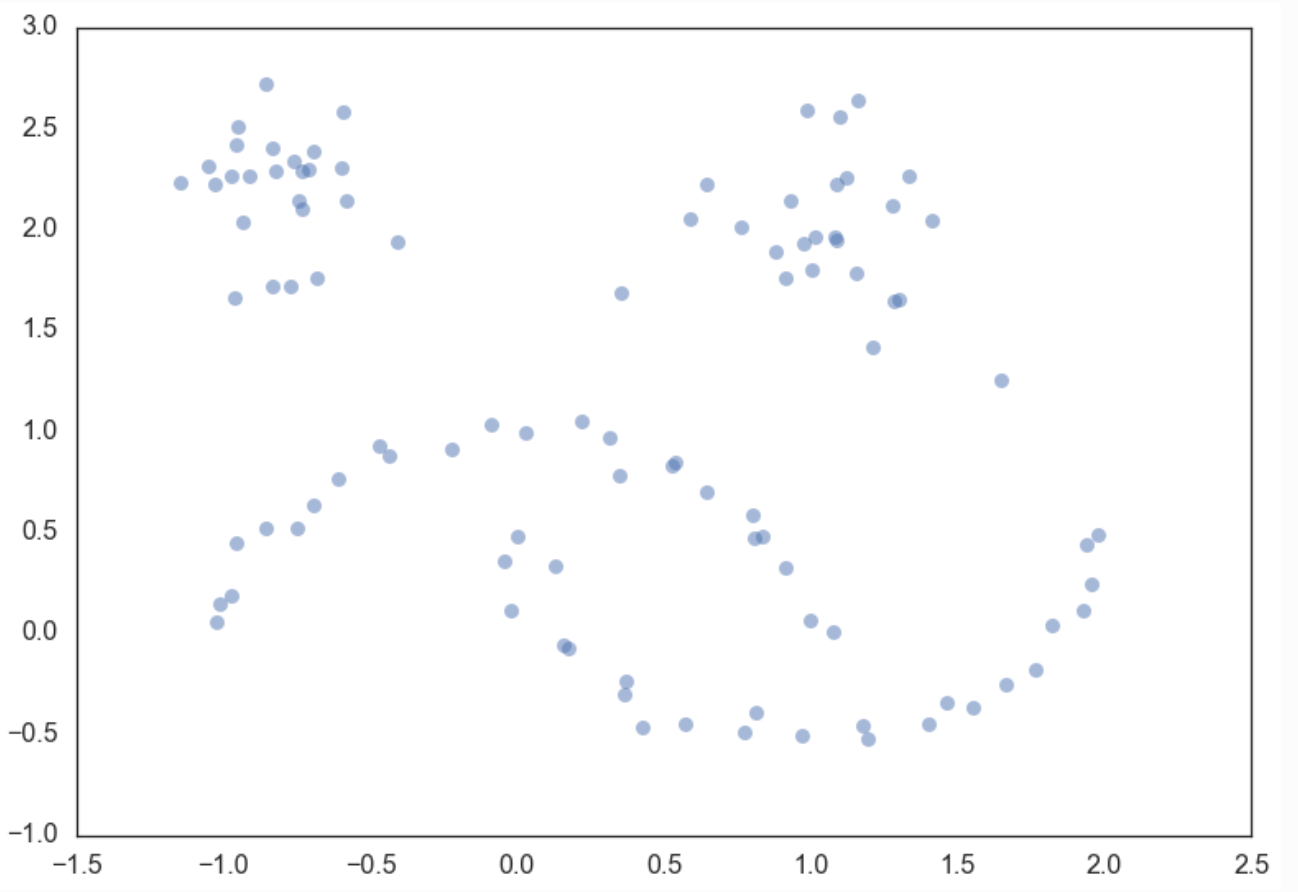
\includegraphics[width=5cm]{image/img_1.png}
\caption{Exemple de distribution de points}
\end{figure}

\textbf{Complexité :} 
\begin{itemize}
\item Stockage des données : $\mathcal{O}(n)$ en mémoire
\item Pré-traitement : $\mathcal{O}(n)$ si normalisation nécessaire
\end{itemize}
\end{frame}

\subsection{2. Vocabulaire de base}

\begin{frame}{2.1 k-ième plus proche voisin}
\begin{block}{Définition}
Pour un point $x \in D$, la \textbf{core distance} (distance de cœur) est :
$$\operatorname{core}_k(x) = d_k'(x)$$
où $d_k'(x)$ est la distance au $k$-ième plus proche voisin.
\end{block}

\textbf{Complexité du calcul :}
\begin{itemize}
\item \textbf{Algorithme naïf :} $\mathcal{O}(n^2)$ pour chaque point $\Rightarrow$ $\mathcal{O}(n^3)$ total
\item \textbf{Avec kd-tree :} $\mathcal{O}(n \log n)$ en moyenne pour $k$ fixe
\item \textbf{Avec LSH :} $\mathcal{O}(n^{1+\rho})$ pour grandes dimensions
\item Implémentation HDBSCAN utilise \texttt{sklearn.neighbors} : $\mathcal{O}(n \log n)$
\end{itemize}
\end{frame}

\begin{frame}{2.1 k-ième plus proche voisin}
\begin{figure}
\centering
% \begin{tikzpicture}[scale=0.7]
% \draw[->] (0,0) -- (4,0) node[right] {$k$};
% \draw[->] (0,0) -- (0,2) node[above] {$d$};
% \draw[thick,blue] (0.5,0.2) -- (1.5,1.8) -- (3.5,0.5);
% \draw[dashed,red] (1.5,0) -- (1.5,1.8);
% \node[red] at (1.5,-0.3) {$k$};
% \end{tikzpicture}
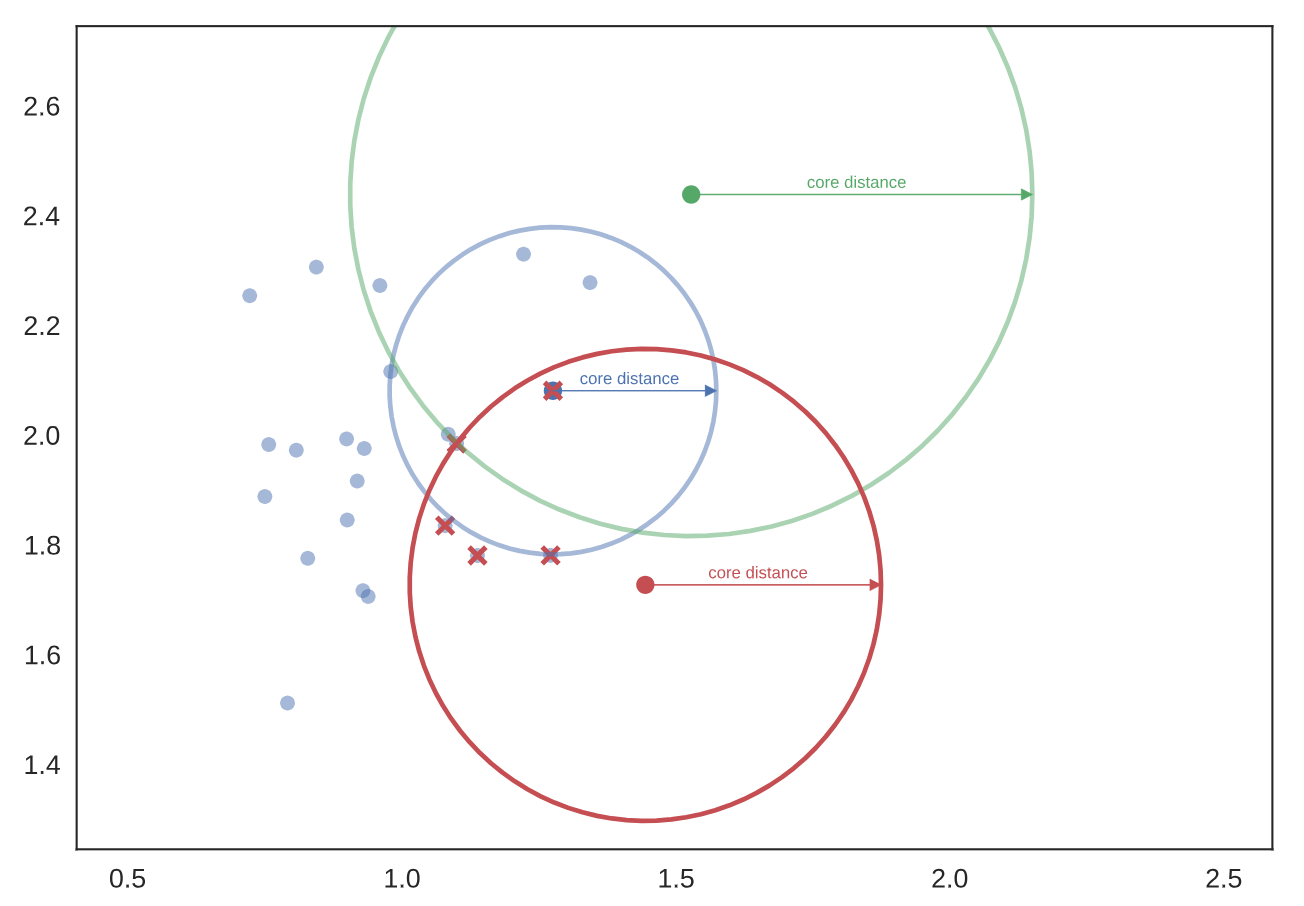
\includegraphics[width=10cm]{image/img_2.png}

\caption{Core distance croit avec $k$}
\end{figure}
\end{frame}

\begin{frame}{2.2 Distance de connectivité mutuelle}
\begin{block}{Définition}
$$d_{\text{mreach-}k}(a,b) = \max\{\operatorname{core}_k(a), \operatorname{core}_k(b), d(a,b)\}$$

\textbf{Propriété de robustesse :}
\begin{itemize}
\item Si $a$ et $b$ denses : $d_{\text{mreach}} \approx d(a,b)$
\item Si $a$ ou $b$ rare : distance forcée à être grande
\item \textbf{Évite les ponts de bruit}
\end{itemize}
\end{block}
\end{frame}

\begin{frame}{2.1 k-ième plus proche voisin}
\begin{figure}
\centering
% \begin{tikzpicture}[scale=0.7]
% \draw[->] (0,0) -- (4,0) node[right] {$k$};
% \draw[->] (0,0) -- (0,2) node[above] {$d$};
% \draw[thick,blue] (0.5,0.2) -- (1.5,1.8) -- (3.5,0.5);
% \draw[dashed,red] (1.5,0) -- (1.5,1.8);
% \node[red] at (1.5,-0.3) {$k$};
% \end{tikzpicture}
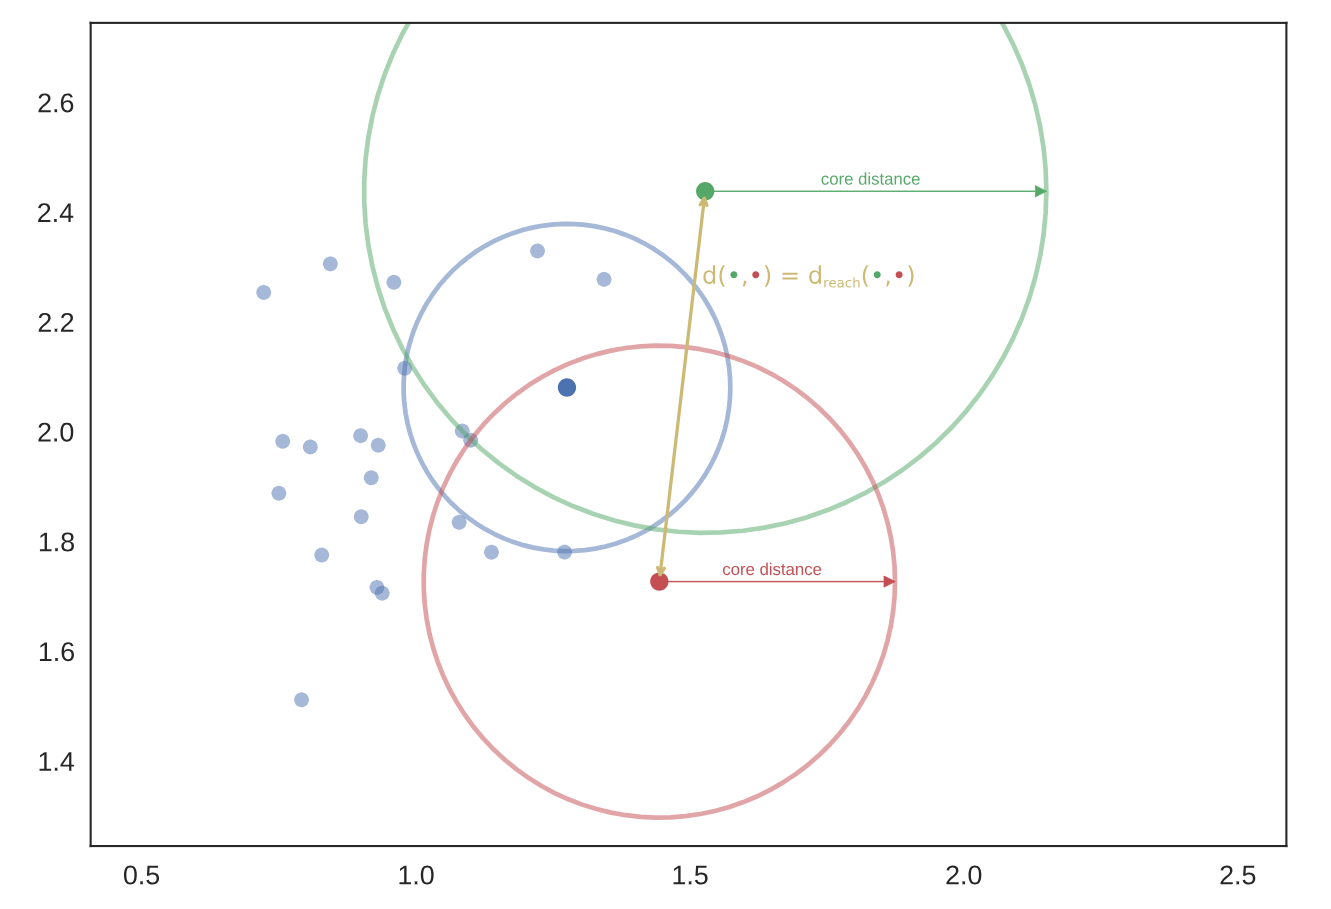
\includegraphics[width=10cm]{image/img_3.png}

\caption{La distance de connectivité mutuelle}
\end{figure}

\textbf{Complexité :} $\mathcal{O}(n^2)$ dans le pire cas pour matrice complète
\end{frame}

\subsection{3. Minimum Spanning Tree (MST)}

\begin{frame}{3. Construction du MST}
\begin{block}{Définition}
Le \textbf{Minimum Spanning Tree} est l'arbre couvrant de poids minimum parmi tous les sous-graphes connexes sans cycles.
\end{block}

\begin{algorithm}[H]
\caption{Algorithme de Prim}
\begin{algorithmic}
\REQUIRE Graphe $G=(V,E)$ connexe et pondéré
\ENSURE Arbre couvrant minimal $T$
\STATE Choisir $s \in V$
\STATE $T \leftarrow \{s\}$
\STATE $C \leftarrow \emptyset$
\WHILE{$T \neq V$}
\STATE Trouver $(u,v)$ de poids minimal avec $u \in T, v \notin T$
\STATE $C \leftarrow C \cup \{(u,v)\}$
\STATE $T \leftarrow T \cup \{v\}$
\ENDWHILE
\RETURN $C$
\end{algorithmic}
\end{algorithm}
\end{frame}

\begin{frame}{3. Construction du MST}
\begin{figure}
\centering
% \begin{tikzpicture}[scale=0.7]
% \draw[->] (0,0) -- (4,0) node[right] {$k$};
% \draw[->] (0,0) -- (0,2) node[above] {$d$};
% \draw[thick,blue] (0.5,0.2) -- (1.5,1.8) -- (3.5,0.5);
% \draw[dashed,red] (1.5,0) -- (1.5,1.8);
% \node[red] at (1.5,-0.3) {$k$};
% \end{tikzpicture}
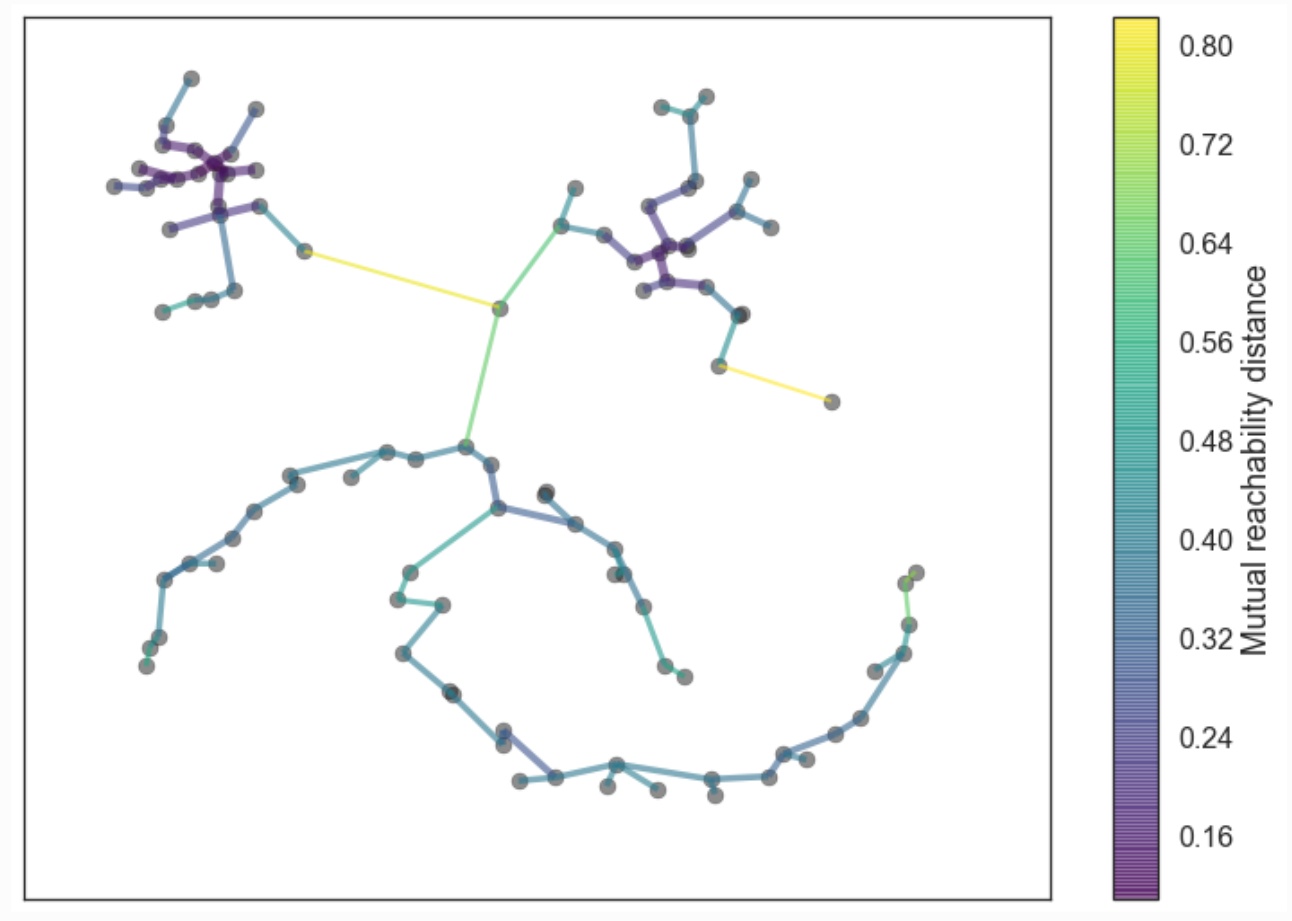
\includegraphics[width=10cm]{image/img_5.png}

\caption{Minimum Spanning Tree}
\end{figure}
\end{frame}

\begin{frame}{Complexité de Prim}
\textbf{Complexités selon la structure de données :}

\begin{center}
\begin{tabular}{|l|c|c|}
\hline
\textbf{Structure} & \textbf{Complexité} & \textbf{Application} \\
\hline
Tableau + parcours linéaire & $\mathcal{O}(n^2)$ & Petits graphes denses \\
\hline
Tas binaire & $\mathcal{O}(E \log V)$ & Graphes classiques \\
\hline
Tas de Fibonacci & $\mathcal{O}(E + V \log V)$ & Graphes très denses \\
\hline
\end{tabular}
\end{center}

\textbf{Dans HDBSCAN :}
\begin{itemize}
\item Graphe complet avec $n$ points : $E = \mathcal{O}(n^2)$
\item Utilisation de Prim optimisé : $\mathcal{O}(n \log n)$ grâce à la \textbf{sparsification}
\item En pratique : $\mathcal{O}(n \log n)$ avec $k$ plus proches voisins limités
\end{itemize}
\end{frame}

\subsection{4. Dendrogramme}

\begin{frame}{4. Clustering Hiérarchique Ascendant}
\begin{algorithm}[H]
\caption{Construction du dendrogramme}
\begin{algorithmic}
\REQUIRE Ensemble $X=\{x_1,\ldots,x_n\}$, distance $d$
\ENSURE Dendrogramme $D$
\STATE $C \leftarrow \{\{x_1\},\ldots,\{x_n\}\}$
\STATE $D \leftarrow \emptyset$
\WHILE{$|C| > 1$}
\STATE Trouver $C_i, C_j$ avec $d(C_i, C_j)$ minimale
\STATE $C_{\text{new}} \leftarrow C_i \cup C_j$
\STATE $h \leftarrow d(C_i, C_j)$ \COMMENT{Hauteur de fusion}
\STATE $D \leftarrow D \cup \{(C_i, C_j, h)\}$
\STATE $C \leftarrow (C \setminus \{C_i, C_j\}) \cup \{C_{\text{new}}\}$
\ENDWHILE
\RETURN $D$
\end{algorithmic}
\end{algorithm}

\textbf{À partir du MST :}
\begin{itemize}
\item Trier les arêtes par poids croissant : $\mathcal{O}(n \log n)$
\item Fusionner progressivement : $\mathcal{O}(n)$ avec Union-Find
\end{itemize}
\end{frame}

\subsection{5. Condensation de l'arbre}

\begin{frame}{5. Condensation de l'arbre de clusters}
\begin{block}{Principe}
Paramètre $m = \text{min\_cluster\_size}$

À chaque division :
\begin{itemize}
\item Si un sous-cluster a $< m$ points $\Rightarrow$ \textbf{points tombent du cluster parent}
\item Si $\geq m$ points $\Rightarrow$ \textbf{vraie division}
\end{itemize}
\end{block}

\begin{figure}
\centering
% \begin{tikzpicture}[scale=0.7, level distance=1cm,
%   level 1/.style={sibling distance=4cm},
%   level 2/.style={sibling distance=2cm}]
% \node {Racine}
%   child {node {Cluster $C_1$ (50 pts)}
%     child {node {Split $C_{1a}$ (45 pts)}}
%     child {node {Split $C_{1b}$ (5 pts)}}
%   }
%   child {node {Bruit}};
% \node[red] at (0,-2.5) {Condensation avec $m=10$};
% \end{tikzpicture}
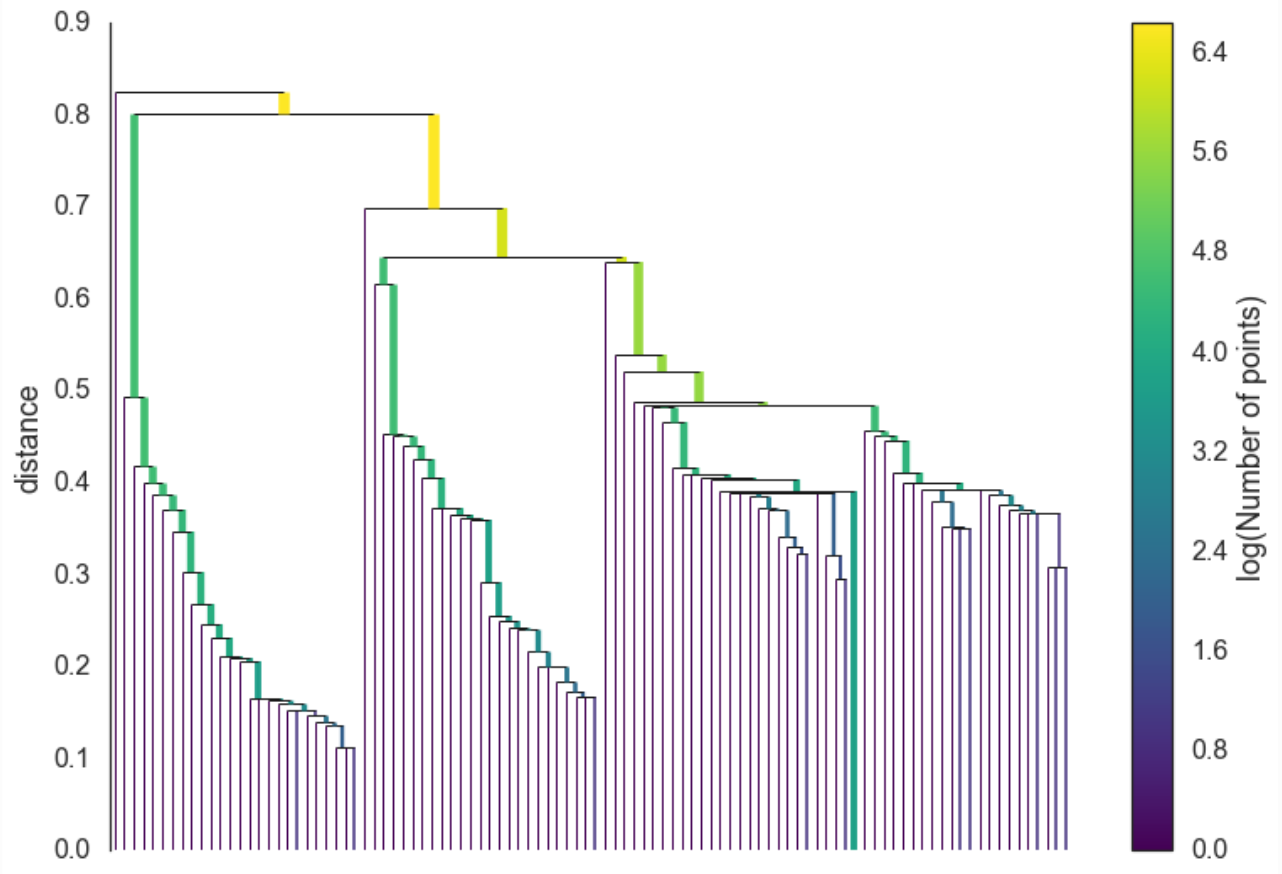
\includegraphics[width=5cm]{image/img_4.png}
\end{figure}

\textbf{Complexité :}
\begin{itemize}
\item Parcours de l'arbre : $\mathcal{O}(n)$ avec structure de fichier plat
\item Mise à jour des compteurs : $\mathcal{O}(n)$
\end{itemize}
\end{frame}

\subsection{6. Extraction des clusters}

\begin{frame}{6.1 Méthode par stabilité}
\begin{block}{Définition de la stabilité}
Pour un cluster avec $\lambda = 1/\text{distance}$ :
\begin{itemize}
\item $\lambda_{\text{birth}}$ : $\lambda$ à la formation
\item $\lambda_{\text{death}}$ : $\lambda$ à la division
\end{itemize}

$$\text{Stabilité} = \sum_{p \in \text{cluster}} (\lambda_p - \lambda_{\text{birth}})$$

Intuition : \textbf{Surface sous la courbe du dendrogramme}
\end{block}

\begin{algorithm}[H]
\caption{Extraction optimale}
\begin{algorithmic}
\STATE Feuilles $\leftarrow$ sélectionnées
\STATE Parcourir ascendant
\IF{Stabilité(enfants) > Stabilité(parent)}
\STATE Propager sélection
\ELSE
\STATE Sélectionner parent, désélectionner enfants
\ENDIF
\end{algorithmic}
\end{algorithm}

\textbf{Complexité :} $\mathcal{O}(n)$ par parcours unique de l'arbre
\end{frame}

\begin{frame}{6. Extraction des clusters}
\begin{figure}
\centering
% \begin{tikzpicture}[scale=0.7]
% \draw[->] (0,0) -- (4,0) node[right] {$k$};
% \draw[->] (0,0) -- (0,2) node[above] {$d$};
% \draw[thick,blue] (0.5,0.2) -- (1.5,1.8) -- (3.5,0.5);
% \draw[dashed,red] (1.5,0) -- (1.5,1.8);
% \node[red] at (1.5,-0.3) {$k$};
% \end{tikzpicture}
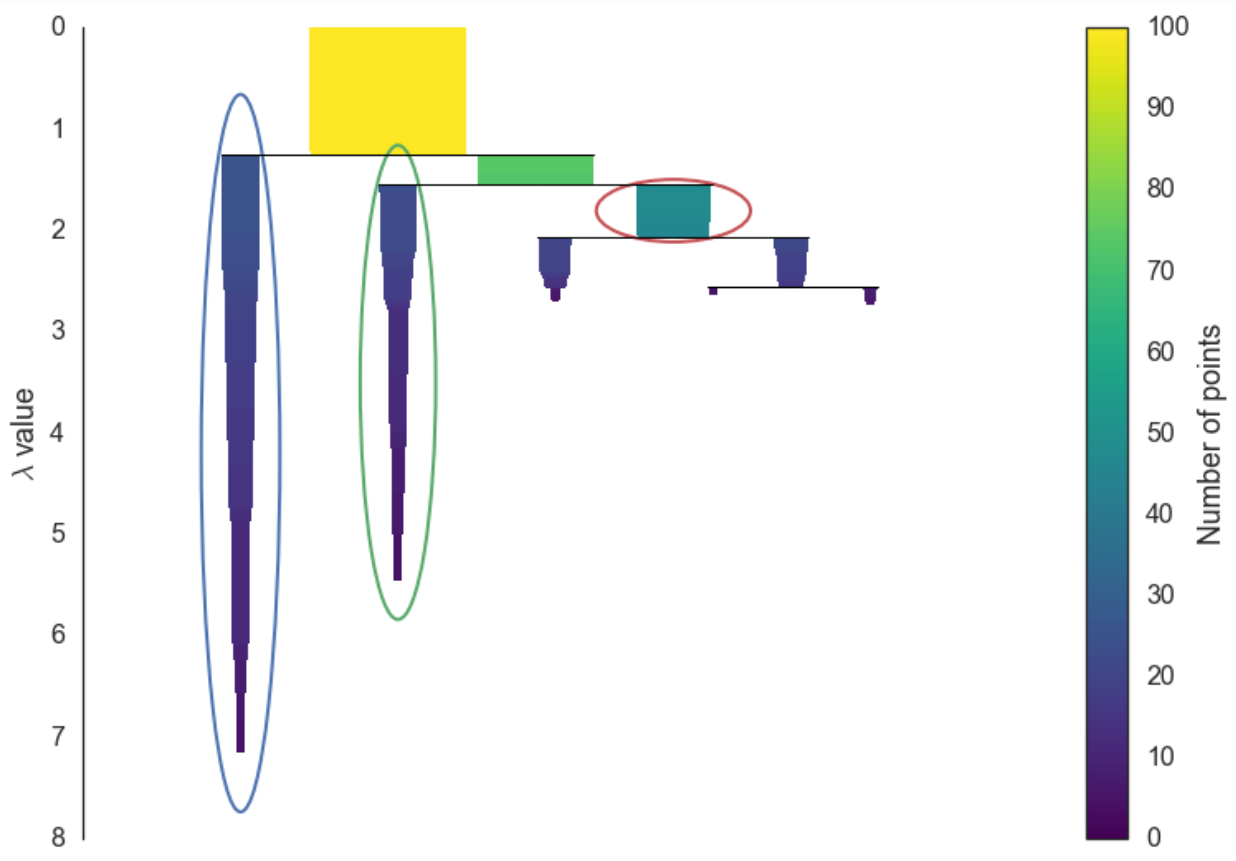
\includegraphics[width=10cm]{image/img_6.png}

\caption{Extraction des clusters}
\end{figure}
\end{frame}

\begin{frame}{6.2 Version simplifiée : Système de percentile}
\begin{block}{Algorithme du gap}
Utilisé dans le package Python \texttt{hdbscan} :

\begin{enumerate}
\item Trier les poids $w_1 \leq w_2 \leq \cdots \leq w_{n-1}$
\item Calculer les écarts $g_i = w_{i+1} - w_i$
\item Trouver $i_{\max} = \arg\max_i g_i$
\item Seuil $\theta = \frac{w_{i_{\max}} + w_{i_{\max}+1}}{2}$
\item Percentile : position de $\theta$ dans la distribution
\end{enumerate}
\end{block}

\begin{figure}
\centering
\begin{tikzpicture}[scale=0.8]
\draw[->] (0,0) -- (5,0) node[right] {$i$};
\draw[->] (0,0) -- (0,2) node[above] {$w_i$};
\draw[thick,blue] (0,0.2) -- (1,0.5) -- (2,0.6) -- (2.5,1.5) -- (3,1.6) -- (4,1.7);
\draw[dashed,red] (2.25,0) -- (2.25,1.55);
\draw[red,thick,<->] (2,1.55) -- (2.5,1.55) node[above,midway] {$g_{\max}$};
\node[red] at (2.25,-0.3) {$\theta$};
\end{tikzpicture}
\end{figure}

\textbf{Complexité :}
\begin{itemize}
\item Tri : $\mathcal{O}(n \log n)$
\item Calcul des écarts : $\mathcal{O}(n)$
\item Extraction par Union-Find : $\mathcal{O}(n \alpha(n))$ (presque linéaire)
\end{itemize}
\end{frame}

\section{Complexité globale}

\begin{frame}{Complexité totale d'HDBSCAN}
\begin{center}
\begin{tabular}{|l|c|}
\hline
\textbf{Étape} & \textbf{Complexité} \\
\hline
k-plus proches voisins & $\mathcal{O}(n \log n)$ (kd-tree) \\
\hline
Distances mutuelles & $\mathcal{O}(n^2)$ (matrice creuse) \\
\hline
Construction du MST & $\mathcal{O}(n \log n)$ (Prim sparse) \\
\hline
Dendrogramme & $\mathcal{O}(n \log n)$ (tri + Union-Find) \\
\hline
Condensation & $\mathcal{O}(n)$ \\
\hline
Extraction (stabilité) & $\mathcal{O}(n)$ \\
\hline
\textbf{TOTAL} & $\mathcal{O}(n \log n)$ à $\mathcal{O}(n^2)$ \\
\hline
\end{tabular}
\end{center}

\begin{alertblock}{Cas pratique}
\textbf{Dominé par le calcul des k-plus proches voisins :}
\begin{itemize}
\item Dim. faible : $\mathcal{O}(n \log n)$ avec kd-tree
\item Dim. élevée : $\mathcal{O}(n^2)$ (malédiction de la dimension)
\item En pratique : $\mathcal{O}(n^{1.5})$ pour $d \approx 10-20$
\end{itemize}
\end{alertblock}
\end{frame}

\section{Comparaison avec DBSCAN}

\begin{frame}{HDBSCAN vs DBSCAN}
\begin{center}
\begin{tabular}{|l|c|c|}
\hline
\textbf{Caractéristique} & \textbf{DBSCAN} & \textbf{HDBSCAN} \\
\hline
Paramètres & $\varepsilon$, $\minPts$ & $\minPts$ seulement \\
\hline
Densité & Uniforme & Variable \\
\hline
Complexité & $\mathcal{O}(n \log n)$ & $\mathcal{O}(n \log n)$ à $\mathcal{O}(n^2)$ \\
\hline
Hiérarchie & Non & Oui \\
\hline
Stabilité & Non & $\mathcal{O}(n)$ \\
\hline
Nombre clusters & Fixé par $\varepsilon$ & Auto-détecté \\
\hline
\end{tabular}
\end{center}

\begin{block}{Trade-off}
\textbf{HDBSCAN} : Plus robuste mais plus coûteux en mémoire ($\mathcal{O}(n^2)$ dans pire cas)
\end{block}
\end{frame}

\section{Implementation pratique}

\begin{frame}{Considérations de performance}
\begin{block}{Optimisations dans \texttt{hdbscan}}
\begin{itemize}
\item \textbf{Approximation des k-NN :} Utilise \texttt{sklearn.neighbors.BallTree}
\item \textbf{Parallélisation :} Calcul des distances sur plusieurs cœurs
\item \textbf{Matrice creuse :} Ne stocke que les $k$ plus proches voisins
\item \textbf{Prim optimisé :} $O(n \log n)$ avec heap
\end{itemize}
\end{block}

\begin{alertblock}{Complexité mémoire}
\begin{itemize}
\item Matrice de distances creuse : $\mathcal{O}(n \cdot k)$
\item MST : $\mathcal{O}(n)$
\item Dendrogramme : $\mathcal{O}(n)$
\end{itemize}
\textbf{Total :} $\mathcal{O}(n \cdot k)$ mémoire ($k \ll n$)
\end{alertblock}
\end{frame}

\section{Conclusion}

\begin{frame}{Résumé}
\begin{itemize}
\item HDBSCAN combine \textbf{densité} et \textbf{hiérarchie}
\item Robustesse via \textbf{distance de connectivité mutuelle}
\item Extraction intelligente par \textbf{stabilité} ou \textbf{gap percentile}
\item Complexité : \textbf{Quasi-linéaire} en dimension faible, $\mathcal{O}(n^2)$ en haute dimension
\end{itemize}

\begin{figure}
\centering
\begin{tikzpicture}[node distance=1.5cm, auto]
\node[block] (data) {Données};
\node[block, right of=data] (knn) {k-NN};
\node[block, right of=knn] (mreach) {Dist. mutuelle};
\node[block, below of=data] (mst) {MST};
\node[block, below of=knn] (dendro) {Dendrogramme};
\node[block, below of=mreach] (extract) {Extraction};
\draw[->] (data) -- (knn);
\draw[->] (knn) -- (mreach);
\draw[->] (mreach) -- (mst);
\draw[->] (mst) -- (dendro);
\draw[->] (dendro) -- (extract);
\end{tikzpicture}
\end{figure}
\end{frame}

\begin{frame}{Références}
\begin{thebibliography}{9}
\bibitem{campello} Campello, R.J.G.B., Moulavi, D., \& Sander, J. \textit{HDBSCAN: Hierarchical Density-Based Spatial Clustering of Applications with Noise}. 2023.

\bibitem{package} Documentation Python : \texttt{https://hdbscan.readthedocs.io/}

\bibitem{complexity} McInnes, L., Healy, J. \textit{Accelerated Hierarchical Density Clustering}, 2017.
\end{thebibliography}

\vspace{1cm}
\centering
\Large\textbf{Merci de votre attention !}
\end{frame}

\end{document}